\documentclass[12pt]{article}
\newcommand\tab[1][0.5cm]{\hspace*{#1}}
\usepackage{graphicx}

\usepackage{hyperref}
\hypersetup{
  colorlinks=true,
  linkcolor=black,
  filecolor=magenta,      
  urlcolor=cyan,
}
\begin{document}

\title{Coding Standards Document}
\maketitle
\center{\textbf{Team Name:} Binary Ninjaz\\}
\center{\textbf{System Name:} Harvest\\}

\includegraphics[scale=0.3]{harvestIcon.png}
\center{\textbf{Client Name:} Barry Christie\\ }{\textbf{Client Affiliation:} Operations Manager at SAMAC\\}
\center{\textbf{Team Members:\\} 
Teboho Mokoena (u14415888)\\
Sizo Duma (u15245579)\\
Letanyan Delon Arumugam (u14228123)\\
John Ojo (u15096794)\\
Kevin Reid (u15008739)\\
Shaun Yates (u16007493)\\ }
\newpage

\tableofcontents
\newpage

\section{Detailed System Design}
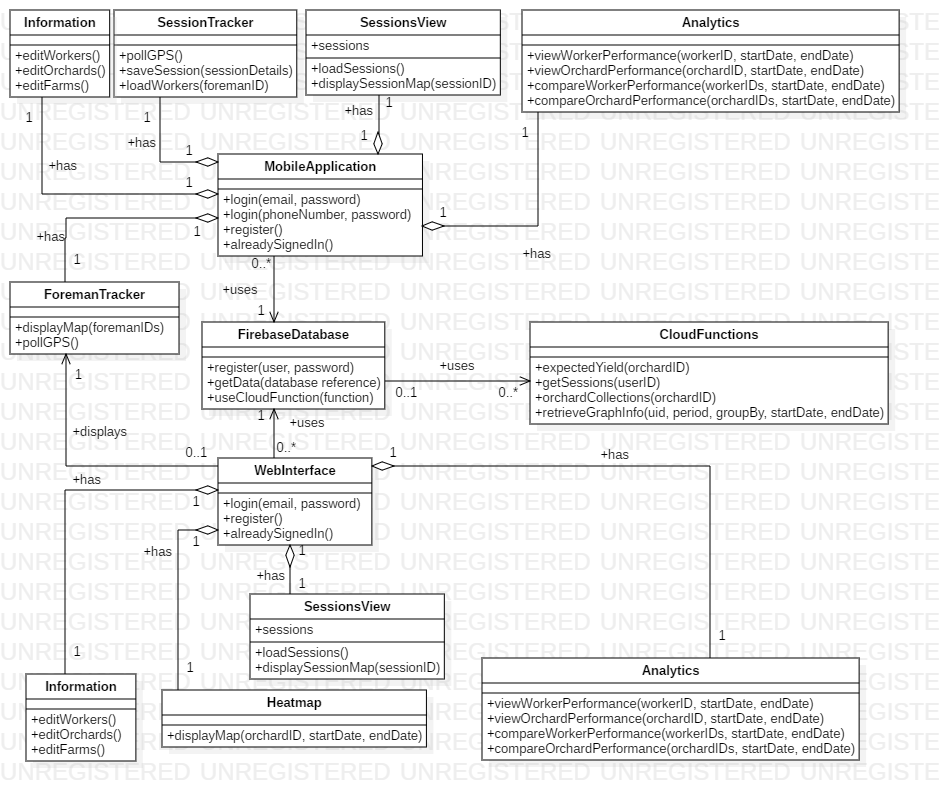
\includegraphics[width=1.2\linewidth]{UMLClassDiag.png}
\newpage

\section{Coding Conventions}
\flushleft
  The project and design we've undertaken means that we will need to use multiple languages and IDE's to complete the project. As such we have decided that the best common practice and standards of each language shall be the standard that is used for that respective language/environment. General coding conventions are used throughout the project and will be listed as well.
  \subsection{HTML/CSS}
  The HTML and CSS standards we shall follow will be the ones of \href{https://google.github.io/styleguide/htmlcssguide.html}{Google's HTML/CSS style guide}
  
  \subsection{JavaScript}
  For JavaScript we will be using \href{https://google.github.io/styleguide/jsguide.html}{Google's JavaScript style guide}.
  
  \subsection{Java}
  Similarly we will use \href{https://google.github.io/styleguide/javaguide.html}{Google's Java style guide}.
  
  \subsection{Swift}
  For Swift we will use \href{https://swift.org/documentation/api-design-guidelines/}{Apple design guidelines}.
  
	\subsection{Other Conventions that are Followed}
Linters are used to enforce many of the rules that we follow, such as:
\item[$\bullet$]Attributes: \newline special @ sign attributes should be on their own line.
\item[$\bullet$]Class Delegate Pattern: \newline Delegate pattern should be implemented using protocols/interfaces. In the case of protocols, the protocol must be a class protocol.
\item[$\bullet$]Closure Closing Indendation: \newline The closures closing brace must end on the same column that the starting lines column is on.\newpage
Incorrect Usage:\newline
  func foo() \{ \newline
   	\tab \} \newline
  Correct Usage: \newline
  func foo() \{ \newline
  \} \newline
\item[$\bullet$]Closure Spacing: \newline Closures must have at least a single space inside of each brace.
\item[$\bullet$]Comma Spacing: \newline A comma must not have any space in front of it and only one space after it.
\item[$\bullet$]Conditional Return Positions: \newline Any return statement from a conditional branch must be on a newline.\newline 
Incorrect Usage:\newline 
  if (true) \{ return 0; \} else \{ return 1; \}\newline 
  Correct Usage:\newline 
  if (true) \{\newline 
   \tab return 0;\newline 
  \} else \{\newline 
   \tab return 1;\newline 
  \}\newline 
  \item[$\bullet$]Cyclomatic Complexity: \newline The cyclomatic complexity of a function body should not exceed more than 10.
  \item[$\bullet$]Singleton Direct Initialization: \newline Singleton classes should not be directly instantiated.
  \item[$\bullet$]Optional Boolean: \newline Where available an Optional may not be used to wrap a Boolean. Prefer an enum instead.
  \item[$\bullet$]Optional Boolean: \newline Where available an Optional may not be used to wrap a Boolean. Prefer an enum instead.
  \item[$\bullet$]Prefer Non-Optional Collection: \newline  Where available an Optional should not be a prefered method of wrapping a collection. Instead try to
  use a collections emptiness to handle nullity as well.
  \item[$\bullet$]Empty Count: \newline Use isEmpty property and not check emptiness via count/length property.
  \item[$\bullet$]Empty Parameter: \newline Prefer Void over an empty parameter.
  \item[$\bullet$]String isEmpty: \newline Prefer using isEmpty over checking equality to an empty string.
  \item[$\bullet$]Avoid Fallthrough: \newline Switch statements should not fallthrough to subsequent cases but instead always break at the end of 
  a case.
  \item[$\bullet$]File Length: \newline File lengths should not exceed more than 2000 lines.
   \item[$\bullet$]File Name: \newline  A file name should match the name of a class/struct/extension it contains.
    \item[$\bullet$]Function Body Length: \newline  Length of a function body should not exceed 150 lines.
     \item[$\bullet$] Default Parameters at End: \newline Default parameters should be the last parameters in a parameter list.
 \item[$\bullet$]Function Parameter Count: \newline A maximum of 5 parameters per function should be allowed.
 \item[$\bullet$]Type Names: \newline Type names should start with an uppercase letter and be of length 1 to 20 characters. Each
  character should only be an alphanumeric. Where subsequent words in the name are also 
  capitilized.
 \item[$\bullet$]Identifier Name: \newline Type names should start with an lowercase letter and be of length 1 to 20 characters. Each
  character should only be an alphanumeric. Where subsequent words in the name are capitilized.
  Or names can be all uppercased if deemed fit.
 \item[$\bullet$] Leading Whitespace: \newline Files may not start with whitespace (excluding comments).
 \item[$\bullet$]Line Length: \newline Lines should not exceed 120 characters.
  \item[$\bullet$]Mark Comments: \newline Mark comments should follow "MARK: ..." or "MARK: -..."
 \item[$\bullet$] Fix Me Comments: \newline Fix me comments should be treated as warnings and follow the format "FIXME: ..."
 \item[$\bullet$] Todo Comments: \newline Todo comments should be treated as warnings and follow the format "TODO: ..."
 \item[$\bullet$] Type Nesting: \newline Types should not be nested more than one type scope deep.
 \item[$\bullet$] Open Brace Spacing: \newline Open braces should be on the same line as the declaration and be preceeded by a single space.
 \item[$\bullet$] Operator Whitespace: \newline Operators should be surrounded by an equal number of whitespace characters.
  \item[$\bullet$] Modify Assign Operators: \newline Prefer operators such as +=, *=, -=, /= over constructs such as `a = a + 42`
  \item[$\bullet$] Redundant Void Return: \newline  Void returning functions should not be explictly stated if not needed.
  \item[$\bullet$] Statement Positions: \newline  Else and catch statements should be on their own line.
  \item[$\bullet$] Switch Case Statement Indentation: \newline  Case statement indentation should be the same as the switch statements indentation. \newline
 Incorrect Usage:\newline
  switch f \{ \newline
    \tab case a: \newline
  \} \newline
  Correct Usage: \newline
  switch f \{ \newline
  case a: \newline
  \} \newline
 \item[$\bullet$] Trailing Newline: \newline Files should have a single newline at the end.
 \item[$\bullet$] Type Body Length: \newline  A types body length should not exceed 500 lines.
 \item[$\bullet$] Unneeded Break: \newline Switch statements should not have unnecessary break statements.
 \item[$\bullet$] Vertical Whitespace: \newline Limit vertical whitespace to a single empty line.
 \newpage
  
\center\section{File Structure}
  \subsection{File Structure Diagram}
  \flushleft 
  \includegraphics[width=1.2\linewidth]{FileStructure.png}
  It is important to note that \texttt{Web/app} is where the main functionality of the website source code can be found and that \texttt{Web/functions} is strictly used for cloud functions.
  
  \center\subsection{Git Branch Structure}
  \includegraphics[width=1.2\linewidth]{GitBranchStructure.png}
  
\flushleft\subsubsection{Branching}
  An example structure is shown above, showing that \texttt{master} is never worked on directly. It is important to note that branch names given of feature branches are not necessarily set branches, but are examples to show branching structure. Each subsystem (Android, iOS, Website) has its own respective branch, and these branches branch off \texttt{Developer}, and in turn any changes done to a branch would then branch off that specific branch. 
  A \texttt{Developer} branch is used, to act in much the same way as \texttt{master}, but as a proxy, so that before merging that branch to master, the entire system can be reviewed there before a more solid commitment is made.
  \subsubsection{Naming}
  \flushleft
  A branch shall never contain an individuals name, rather it must be informative as to what the intention of the branch is whilst also remaining short. An example of a  name that would be deemed unacceptable is \texttt{Joe}; another would be \texttt{JoeWebsiteChanges}, where the name contains a member name, and gives very little information as to what is going on in the branch. Bad, but barely acceptable names are \texttt{WebsiteChanges}, or \texttt{WebsiteExperimentation}. Ideal names are as follows: in the case of a branch where the website is ultimately being assembled, by merging other branches into it, and the only modifications taking place are to structure the files, or a quick fix, such as changing the colour of a button, \texttt{Website}; in the case that a new homepage is created for the website, where the homepage is created, and merged into \texttt{Website} on completion, \texttt{Website-Homepage}. Finally, if a user wants to propose a change to the \texttt{Website-Homepage} branch, where he wants to change the colour of a button, but the user has not been assigned, or is not the primary benefactor to \texttt{Website-Homepage}, he creates a new \texttt{Website-Homepage-ButtonColourChange} branch. Notice that in the ideal examples it is possible to track down the source of a branch, to understand exactly what it's purpose is.
  
  \newpage
  \center\section{Code Review Process}
  \flushleft
All code reviewing is done on GitHub, and occurs every time there are changes done to code, or if new code has been implemented. Currently, pre-commit reviews are utilized and although it is a slower process compared to post-commit reviews, it always for more people to be aware of changes to the code and could possibly lead to better implementation as more eyes usually means more ideas. \newline
After changes have been made on the branch, the creator, who wants to merge, will then make a pull request on GitHub, and announce the request on Slack. After which it shall become the responsibility of the entire team, but more importantly that of the original branch maintainer to analyze and comment on the changes. The exact location of the discussion is trivial, however GitHub provides a better, and more concrete platform for this discussion to take place, where inline comments can be made. After a sufficient amount of time and discussion has passed, either the branch maintainer (if it is a minor change), or the entire team (if it is to master, or a major change) shall decide to merge or not.

  
\end{document}